\exercise

2. 利用$1+x+\cdots +x^n$的求和公式,求出下列各式的和:
\begin{tasks}(1)
    \task $1+2x+3x^2+\cdots+nx^{n-1}$;
    \task $\displaystyle\sum_{k=1}^n \displaystyle\frac{k}{2^{k-1}}$;
    \task $1^2+2^2 x + 3^2 x^2 + \cdots + n^2 x^{n-1}$.
\end{tasks}

(1) \solve 令原式等于$S(n)$,利用裂项相消法:
\begin{align}
    S(n) - x S(n) &= (1-x)S(n) \\
    &= \sum_{k=1}^n k x^{k-1} - x \sum_{k=1}^{n} k x^{k-1} \\
    &= \sum_{k=1}^n k x^{k-1} - \sum_{k=1}^{n} k x^k \\
    &= 1 + \sum_{k=2}^{n} k x^{k-1} - \sum_{k=1}^{n} kx^{k} \\
    &= 1 + \sum_{k=1}^{n-1} (k+1) x^k - \sum_{k=1}^{n} k x^{k} \\
    &= 1 - n x^n + \sum_{k=1}^{n-1} (k+1) x^k - \sum_{k=1}^{n-1} k x^{k} \\
    &= 1 - nx^n + \sum_{k=1}^{n-1} x^k \\
    &= 1 - nx^n + x \sum_{k=1}^{n-1} x^{k-1} \\
    &= 1 - nx^n + x \cdot \frac{1-x^{n-1}}{1-x}
\end{align}
于是有
\begin{align}
    S(n) &= \frac{(1-x)S(n)}{1-x} \\
    &= \frac{1-nx^n}{1-x} + x \cdot \frac{1-x^{n-1}}{(1-x)^2}.
\end{align}
\qed\bigskip

(2) \solve 代入题(1)的结论即可:
\begin{align}
    \sum_{k=1}^{n} \frac{k}{2^{k-1}} &= \sum_{k=1}^n k \cdot \left( \frac{1}{2} \right)^{k-1} \\
    &= \frac{1}{2} + 2 \cdot \left(\displaystyle\frac{1}{2}\right) + 3 \cdot \left(\displaystyle\frac{1}{2}\right)^2 + \cdots + n \cdot \left(\displaystyle\frac{1}{2}\right)^{n-1} \\
    &= \frac{1 - n \left(\displaystyle\frac{1}{2}\right)^n}{1 - \displaystyle\frac{1}{2}} + \left(\displaystyle\frac{1}{2}\right) \cdot \frac{1 - \left(\displaystyle\frac{1}{2}\right)^{n-1}}{\left(1-\displaystyle\frac{1}{2}\right)^2}.
\end{align}
\qed\bigskip

(3) \solve 令原式为$S(n)$,采用裂项相消法:
\begin{align}
    S(n) - xS(n) &= (1-x)S(n) \\
    &= \sum_{k=1}^n k^2 x^{k-1} - x \sum_{k=1}^{n} k^2 x^{k-1} \\
    &= 1 + \sum_{k=2}^{n} k^2 x^{k-1} - \sum_{k=1}^{n} k^2 x^k \\
    &= 1 - n^2 x^n + \sum_{k=1}^{n-1} (k+1)^2 x^k - \sum_{k=1}^{n-1} k^2 x^k \\
    &= 1 - n^2 x^n + \sum_{k=1}^{n-1} \left((k+1)^2 - k^2 \right) x^k \\
    &= 1 - n^2 x^n + \sum_{k=1}^{n-1} \left(2k + 1 \right) x^k \\
    &= 1 - n^2 x^n + \sum_{k=2}^{n} \left(2k - 1 \right) x^{k-1} \\
    &= \left(\sum_{k=1}^{n} \left(2k - 1 \right) x^{k-1} \right) - n^2 x^n 
\end{align}
令
\begin{equation}
    P(n) = \sum_{k=1}^n k x^{k-1}, \quad Q(n) = \sum_{k=1}^n x^{k-1}
\end{equation}
那么
\begin{align}
    2P(n)-Q(n) &= 2 \sum_{k=1}^n k x^{k-1} - \sum_{k=1}^n x^{k-1} \\
    &= \sum_{k=1}^n 2k x^{k-1} - \sum_{k=1}^n x^{k-1} \\
    &= \sum_{k=1}^n (2k-1) x^{k-1}
\end{align}
那么
\begin{align}
    (1-x)S(n) &= \left(\sum_{k=1}^{n} \left(2k - 1 \right) x^{k-1} \right) - n^2 x^n \\
    &= 2P(n) - Q(n) - n^2 x^n
\end{align}
从而
\begin{equation}
    S(n) = \frac{2P(n)-Q(n)-n^2 x^n}{1-x}.
\end{equation}
\qed\bigskip

3. 证明组合恒等式:
\begin{tasks}(1)
    \task $\displaystyle\sum_{k=1}^n k \binom{n}{k} = n 2^{n-1} \; (n \in \nat)$;
    \task $\displaystyle\sum_{k=1}^n k^2 \binom{n}{k} = n(n+1)2^{n-2} \; (n \in \nat)$.
\end{tasks}

(1) \prove 令$S(n) = \displaystyle\sum_{k=1}^{n} k \binom{n}{k}$,则
\begin{align}
    \text{左边} &= \sum_{k=1}^{n} k \binom{n}{k} \\
    &= S(n) \\
    &= S(n) - S(n-1) + S(n-1) \\
    &= (S(n) - S(n-1)) + S(n-1)
\end{align}
我们先来算$S(n)-S(n-1)$,看它等于多少:
\begin{align}
    \text{它} &= S(n) - S(n-1) \\
    &= \sum_{k = 1}^{n} k \binom{n}{k} - \sum_{k = 1}^{n-1} k \binom{n-1}{k} \\
    &= n \binom{n}{n} + \sum_{k=1}^{n-1} k \left(\binom{n}{k} - \binom{n-1}{k}\right) \\
    &= n \binom{n}{n} + \sum_{k=1}^{n-1} k \binom{n-1}{k-1} \\
    &= n + \binom{n-1}{0} + 2 \binom{n-1}{1} + \cdots + (n-2)\binom{n-1}{n-3} + (n-1)\binom{n-1}{n-2}
\end{align}
我们再来看$S(n-1)$等于多少:
\begin{align}
    S(n-1) &= \sum_{k=1}^{n-1} k \binom{n-1}{k} \\
    &= \binom{n-1}{1} + 2\binom{n-1}{2} + \cdots + (n-2)\binom{n-1}{n-2} + (n-1)\binom{n-1}{n-1} \\
    &= (n-1) \binom{n-1}{n-1} + (n-2)\binom{n-1}{n-2} + \cdots + 2 \binom{n-1}{2} + \binom{n-1}{1} \\
    &= (n-1) \binom{n-1}{0} + (n-2)\binom{n-1}{1} + \cdots + 2 \binom{n-1}{n-3} + \binom{n-1}{n-2}
\end{align}
所以$S(n)-S(n-1)$加上$S(n-1)$就等于:
\begin{align}
    &\mathrel{\phantom{=}} S(n) - S(n-1) + S(n-1) \\
    &= n + \binom{n-1}{0} + 2 \binom{n-1}{1} + \cdots + (n-2)\binom{n-1}{n-3} + (n-1)\binom{n-1}{n-2} \\
    &+ (n-1) \binom{n-1}{0} + (n-2)\binom{n-1}{1} + \cdots + 2 \binom{n-1}{n-3} + \binom{n-1}{n-2} \\
    &= n + n \binom{n-1}{0} + n \binom{n-1}{1} + \cdots + n\binom{n-1}{n-2} \\
    &= n + n (\binom{n-1}{0} +  \binom{n-1}{1} + \cdots + \binom{n-1}{n-2} + \binom{n-1}{n-1}) - n\binom{n-1}{n-1} \\
    &= n (\binom{n-1}{0} +  \binom{n-1}{1} + \cdots + \binom{n-1}{n-2} + \binom{n-1}{n-1}) \\
    &= n 2^{n-1}.
\end{align}
这就证明了$S(n) = n 2^{n-1}$.\qed\bigskip

(2) \prove 采用数学归纳法.当$n=1$时
\begin{align}
    \text{左边} &= \sum_{k=1}^1 k^2 \binom{n}{k} = 1 \binom{1}{1} = 1 = 1(1+1) 2^{1-2} = \text{右边}.
\end{align}
也就是说当$n=1$时待证等式成立.

对一般的$n \in \nat$,令
\begin{equation}
    S(n) = \sum_{k=1}^n k^2 \binom{n}{k}
\end{equation}
于是我们有
\begin{align}
    S(n) &= \sum_{k=1}^{n} k^2 \binom{n}{k} = n^2 + \sum_{k=1}^{n-1} k^2 \binom{n}{k} \\
    &= n^2 + \sum_{k=1}^{n-1} k^2 \binom{n-1}{k-1} + \sum_{k=1}^{n-1} k^2 \binom{n-1}{k} \\
    &= n^2 + \sum_{k=1}^{n-1} k^2 \binom{n-1}{k-1} + S(n-1) \\
    &= \sum_{k=0}^{n-1} (k+1)^2 \binom{n-1}{k} + S(n-1)
\end{align}
于是
\begin{equation}
    S(n) - S(n-1) = \sum_{k=0}^{n-1} (k+1)^2 \binom{n-1}{k}
\end{equation}
于是
\begin{align}
    S(n) - S(n-1) - S(n-1) &= \sum_{k=0}^{n-1} (k+1)^2 \binom{n-1}{k} - \sum_{k=1}^{n-1} k^2 \binom{n-1}{k} \\
    &= \binom{n-1}{0} + \sum_{k=1}^{n-1} \left((k+1)^2 - k^2\right) \binom{n-1}{k} \\
    &= \binom{n-1}{0} + \sum_{k=1}^{n-1} \left(2k + 1\right) \binom{n-1}{k} \\
    &= \sum_{k=0}^{0} \left(2k+1\right) \binom{n-1}{k} + \sum_{k=1}^{n-1} \left(2k+1\right) \binom{n-1}{k} \\
    &= \sum_{k=0}^{n-1} \left(2k+1\right) \binom{n-1}{k} = \sum_{k=1}^{n} \left(2k-1\right) \binom{n-1}{k-1} \\
    &= \sum_{k=0}^{n-1} (2k+1) \binom{n-1}{k} = \sum_{k=0}^{n-1} \binom{n-1}{k} + 2\sum_{k=0}^{n-1}k \binom{n-1}{k} \\
    &= \sum_{k=0}^{n-1} \binom{n-1}{k} + 2 \sum_{k=1}^{n-1} k \binom{n-1}{k} \\
    &= 2^{n-1} + 2 (n-1) 2^{n-2} = n 2^{n-1}
\end{align}
从而我们得
\begin{equation}
    S(n) - S(n-1) = n 2^{n-1} + S(n-1)
\end{equation}
对一般的$n \in \nat$都成立(注意:这个式子和归纳假设无关!).下面,假设对于某个整数$k \in \nat$,有
\begin{equation}
    S(k) = k(k+1)2^{k-2}
\end{equation}
成立,那么
\begin{align}
    S(k+1) &= S(k) + S(k+1) - S(k) = k(k+1) 2^{k-2} + (k+1)2^{k} + k(k+1)2^{k-2} \\
    &= (k+2)(k+1)2^{k-1}.
\end{align}
从而式子$S(n) = n(n+1)2^{n-2}$对一般的$n \in \nat$都成立.\qed\bigskip

4. 若$f$是一个可导的周期函数,试证:$f^\prime$也是周期函数.

\prove 设$l > 0$是$f$的一个周期长度,任取$x_1 \in \real$,我们知道$f^{\prime}(x_0)$是存在的,下面来计算$f^{\prime}(x_0 + l)$,依定义:
\begin{align}
    f^{\prime}(x_0 + l) &= \lim_{h \to 0} \frac{f(x_0+l+h)-f(x_0+l)}{h} \\
    &= \lim_{h \to 0} \frac{f(x_0+h + l)-f(x_0)}{h} \\
    &= \lim_{h \to 0} \frac{f(x_0+h)-f(x_0)}{h} \\
    &= f^{\prime}(x_0).
\end{align}
这足以说明$f^{\prime}$是周期的.\qed\bigskip

5. 证明:
\begin{tasks}(1)
    \task 若$f$是可导的奇函数,则$f^\prime$是偶函数;
    \task 若$f$是可导的偶函数,则$f^\prime$是奇函数.
\end{tasks}
对以上命题做几何解释.

(1) \prove 任取$x_0 \in \real$,依定义
\begin{align}
    f^{\prime}(-x_0) &= \lim_{h \to 0} \frac{f(-x_0 + h) - f(-x_0)}{h} \\
    &= \lim_{h \to 0} \frac{f(-(x_0-h))-(-f(x_0))}{h} \\
    &= \lim_{h \to 0} \frac{-f(x_0-h)+f(x_0)}{h} \\
    &= \lim_{-h \to 0} \frac{f(x_0 - h)-f(x_0)}{-h} \\
    &= \lim_{-h \to 0} \frac{f(x_0 + (- h))-f(x_0)}{-h} \\
    &= f^{\prime}(x_0).
\end{align}
从而若$f$是奇的,则$f^{\prime}$是偶的.\qed\bigskip

(2) \prove 任取$x_0 \in \real$,依定义
\begin{align}
    f^{\prime}(-x_0) &= \lim_{h \to 0} \frac{f(-x_0+h)-f(-x_0)}{h} \\
    &= \lim_{h \to 0} \frac{f(h-x_0)-f(x_0)}{h} \\
    &= \lim_{h \to 0} \frac{f(x_0-h)-f(x_0)}{h} \\
    &= \lim_{-h \to 0} \frac{f(x_0+(-h))-f(x_0)}{-(-h)} \\
    &= \lim_{-h \to 0} -\frac{f(x_0+(-h))-f(x_0)}{-h} \\
    &= -\lim_{-h \to 0} \frac{f(x_0+(-h))-f(x_0)}{-h} \\
    &= -f^{\prime}(x_0).
\end{align}
从而若$f$是偶的,则$f^{\prime}$是奇的.\qed\bigskip

\textbf{解释.} 偶函数的图像是关于$y$轴对称的,因此在$x > 0$处的函数图像和$x<0$处的函数图像的爬升趋势(斜率)总是相反的,这就解释了为什么偶的$f$总有奇的$f^{\prime}$.奇函数的图像是始终上升的,因此如果在$x < 0$的切线的斜率是正的,那么它在$-x > 0$的切线的斜率也还得是正的,故$f^{\prime}$是偶的.\qed\bigskip

6. 设$f$是一个三次多项式,且$f(a)=f(b)=0$.证明:函数$f$在$[a,b]$上不变号的充分必要条件是$f^{\prime}(a)f^{\prime}(b)\leq 0$.

\prove 

必要性.

若$f$在$[a,b]$恒为$0$结论显然成立,现在不失一般性假设$\forall x \in (a,b), f(x) > 0$.现计算$f^{\prime}_{+}(a)$,它等于
\begin{equation}
    \lim_{h \to 0^+} \frac{f(a+h)-f(a)}{h} > 0
\end{equation}
再计算$f^{\prime}_{-}(b)$,它等于
\begin{equation}
    \lim_{h \to 0^-} \frac{f(b+h)-f(b)}{h} < 0
\end{equation}
依连续性知$f^{\prime}(a)=f^{\prime}_{+}(a), f^{\prime}(b)=f^{\prime}_{-}(b)$,从而$f^{\prime}(a)f^{\prime}(b) < 0$.

充分性.

采用反证法.假设存在$x_1, x_2 \in (a,b)$且$x_1 < x_2$使得$f(x_1)f(x_2)<0$,那么由连续性,存在$c \in (x_1,x_2)$使得$f(c)=0$,由于$f$是$3$次多项式,最多只能有$3$个实根,故在$a,b,c$这三点之外$f(x)$都不等于$0$.由于$f(x_1)$与$f(x_2)$异号,不失一般性可以假设$f(x_1) > 0$且$f(x_2)<0$.因为若能在$(a,c)$找到两点使$f(x)$异号那么根据连续性就能得出有第四个根显然这是不可能的,同理也不可能在$(c,b)$中找到两点使$f(x)$异号,从而对任意$x \in (a,c)$,有$f(x) > 0$,对任意$ x \in (c, b)$,有$f(x) < 0$.从而$f^{\prime}(a) > 0$并且$f^{\prime}(b)>0$,从而$f^{\prime}(a)f^{\prime}(b)>0$,矛盾.\qed\bigskip

7. 设函数$f$在$[a,b]$上连续,$f(a)=f(b)=0$,且
\begin{equation*}
    f^{\prime}_{+}(a)f^{\prime}_{-}(b)>0
\end{equation*}
证明:$f$在$(a,b)$内至少有一个零点.

\prove 采用反证法.假设$f$在$(a,b)$内没有零点.任取$x_1 \in (a,b)$,不妨设$f(x_1)>0$,则对所有$x \in (a,b)$都有$f(x)>0$,否则根据零值定理可在$(a,b)$中找到零点(与假设不符).由于对任意$x \in (a,b)$都有$f(x)>0$,由此推出$f^{\prime}_{+}(a)>0$且$f^{\prime}_{-}(b)<0$,从而$f^{\prime}_{+}(a)f^{\prime}_{-}(b)<0$,矛盾.\qed\bigskip

8. 证明:双曲线$xy=a>0$在各点处的切线与两坐标轴所围成的三角形的面积为常数.

\prove 任取$x_0 > 0$,设$(x_0,y_0)$是该双曲线上一点,设过$(x_0,y_0)$的切线与$y$轴交于$A$,与$x$轴交于$B$,设点$(x_0,y_0)$在$y$轴上的投影为$C=(0,y_0)$,在$x$轴上的投影为$D=(x_0,0)$.设坐标系原点为$O$,于是该点的切线与坐标轴围成的三角形为$\triangle AOB$.面积为$\displaystyle\frac{1}{2}\lvert AO \rvert \lvert OB \rvert$.先来计算$\lvert AO \rvert$.设该切线的斜率为$k$.
\begin{align}
    \lvert AO \rvert &= \lvert OC \rvert + \lvert CA \rvert = y_0 + x_0 \lvert k \rvert \\
    &= y_0 + x_0 \cdot \frac{a}{x_0^2} = y_0 + \frac{a}{x_0}
\end{align}
再来计算$\lvert OB \rvert$:
\begin{align}
    \lvert OB \rvert &= \lvert OD \rvert + \lvert DB \rvert \\
    &= x_0 + y_0 \div \lvert k \rvert \\
    &= x_0 + \frac{x_0^2 y_0}{a}
\end{align}
再来计算面积:
\begin{align}
    \mathrm{S}(\triangle AOB) &= \frac{1}{2} \lvert AO \rvert \lvert OB \rvert \\
    &= \frac{1}{2} \left(y_0 + \frac{a}{x_0}\right)\left(x_0+\frac{x_0^2y_0}{a}\right) \\
    &= \frac{1}{2} \left(y_0 x_0 + \frac{x_0^2y_0^2}{a} + a + x_0y_0\right) = 2a.
\end{align}
该面积的确为常数.\qed\bigskip

9. 证明抛物线的光学性质:若光源置于抛物线的焦点上,则其经过抛物线镜面的反射之后,成为一束平行于抛物线的对称轴的光线.

\prove 考虑抛物线$y = x^2$,它的焦点位于$(0, \displaystyle\frac{1}{4})$.设竖直光线$x = x_0 \; (x_0 > 0)$与抛物线交于点$A(x_0, x_0^2)$,设点$A$在$x$轴上的投影为$B(x_0, 0)$,设点$A$处的切线与$x$轴交于点$C$,设切线的斜率是$k$,那么依几何关系,我们有
\begin{equation}
    \frac{\lvert AB \rvert}{\lvert BC \rvert} = \lvert k \rvert = 2x_0
\end{equation}
代入$\lvert AB \rvert = x_0^2$,解从$\lvert BC \rvert = \displaystyle\frac{x_0}{2}$,从而得点$C$坐标$(\displaystyle\frac{x_0}{2},0)$.设点$S$是光线上足够高的一点$(x_0, M_1) \; M_1 > 0$,点$R$是切线上足够高的一点,则角$\angle SAR$为入射角,记为$\alpha$,依几何关系,我们知$\angle CAB = \angle SAR = \alpha$.设光线经过点$A$的反射于$y$轴交于$D$,那么$\angle DAC$为反射角,根据光的反射规律我们知$\angle DAC = \alpha$,从而$\angle DAB = \angle DAC + \angle CAB = 2\alpha$.我们要证这个点$D$就是焦点.

过点$D$做直线$AB$上的垂线,设垂足为$G$,由于$D$是$y$轴上的,$G$是光线上的,光线是垂直射入的,所以很容易知道$\lvert DG \rvert = x_0$,由几何关系,我们知
\begin{equation}
    \frac{\lvert DG \rvert}{\lvert AG \rvert} = \tan \, \angle DAG = \tan \, 2\alpha
\end{equation}
又根据几何关系,我们知
\begin{equation}
    \begin{cases}
        \displaystyle\frac{\lvert AB \rvert}{\lvert BC \rvert} &= k = 2x_0 \\
        \displaystyle\frac{\lvert BC \rvert}{\lvert AB \rvert} &= \tan \, \alpha
    \end{cases}
\end{equation}
这也就是说$\tan \, \alpha = \displaystyle\frac{1}{2x_0}$,利用正切的二倍角公式我们有
\begin{equation}
    \lvert AG \rvert = \frac{\lvert DG \rvert}{\tan \, 2 \alpha} = \frac{x_0}{\tan \, 2 \alpha} = \frac{x_0(1-\tan^2 \, \alpha)}{2 \tan \, \alpha}
\end{equation}
那么
\begin{equation}
    \lvert BG \rvert = \lvert BA \rvert - \lvert AG \rvert = x_0^2 - \frac{x_0(1-\tan^2 \, \alpha)}{2 \tan \, \alpha}
\end{equation}
代入$\tan \, \alpha = \displaystyle\frac{1}{2x_0}$就算得
\begin{equation}
    \lvert BG \rvert = \frac{1}{4}
\end{equation}
这说明$D$位于焦点.\qed\bigskip

\begin{figure}[H]
    \centering
    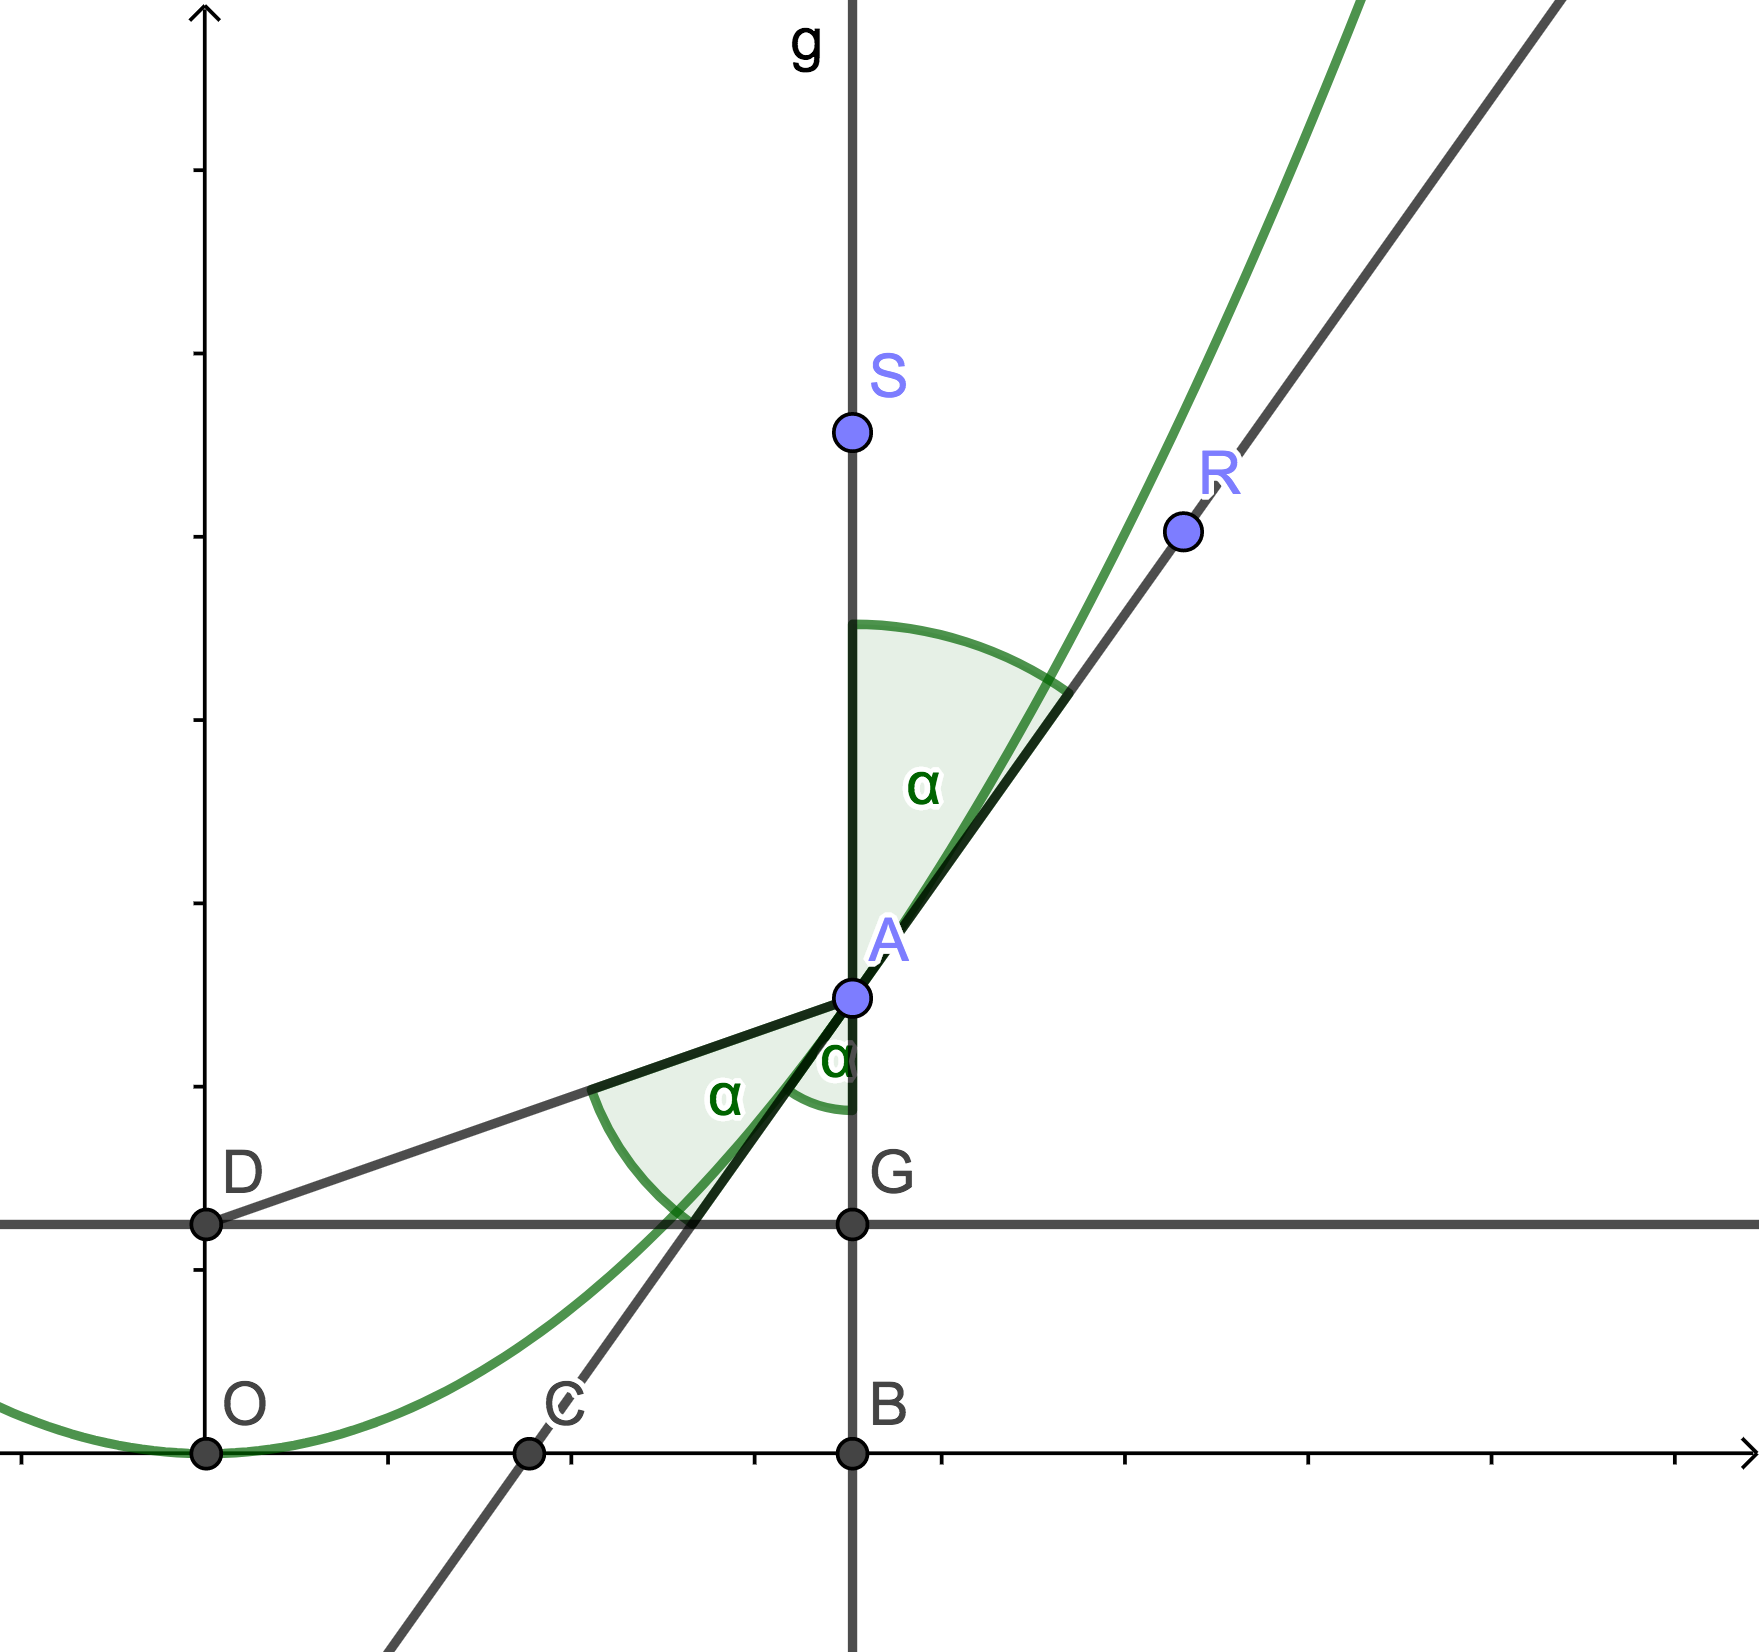
\includegraphics[width=0.45\textwidth]{chapter3/light.png}
    \caption{抛物线证明题图示}
\end{figure}

10. 水来自高为\SI{18}{\centi\metre}、底半径为\SI{6}{\centi\metre}的圆锥型漏斗流入直径为\SI{10}{\centi\metre}的圆柱形桶内.已知漏斗水深\SI{12}{\centi\metre}时,水面下降的速度为\SI{1}{\centi\metre/\second},求此时桶中水面上升的速度.

\solve 在每时每刻流入桶中的水的体积和流出漏斗的水的体积是相等的,设漏斗水面下降的速度为$v_1$,设水桶水面上升的速度为$v_2$,设漏斗水面的面积为$A_1$,设水桶水面的面积为$A_2$,那么应有
\begin{equation}
    A_1 v_1 = A_2 v_2
    \label{eq:3-2-102}
\end{equation}
设漏斗此刻的水面的半径是$x \; \si{\centi\metre}$,那么根据几何关系
\begin{equation}
    \frac{x}{12} = \frac{6}{18}
\end{equation}
解出$x=4$,桶面直径是$10 \; \si{\centi\metre}$,所以桶面半径是$5 \; \si{\centi\metre}$,从而
\begin{equation}
    \begin{cases}
        A_1 = \pi 4^2 \; (\si{\centi\metre^2}) \\
        A_2 = \pi 5^2 \; (\si{\centi\metre^2})
    \end{cases}
\end{equation}
我们已经知道$v_1 = 1 \; (\si{\centi\metre/\second})$,把上式代入式(\ref{eq:3-2-102})立即解出
\begin{equation}
    v_2 = \frac{A_1 v_1}{A_2} = \frac{\pi 4^2 \cdot 1}{\pi 5^2} \; (\si{\centi\metre/\second}) = 0.64 \; (\si{\centi\metre/\second}).
\end{equation}
\qed\bigskip